\documentclass{beamer}
\usetheme{Madrid} % My favorite!
%\usetheme{Boadilla} % Pretty neat, soft color.
%\usetheme{default}
%\usetheme{Warsaw}
%\usetheme{Bergen} % This template has nagivation on the left
%\usetheme{Frankfurt} % Similar to the default 
%with an extra region at the top.
%\usecolortheme{seahorse} % Simple and clean template
%\usetheme{Darmstadt} % not so good
% Uncomment the following line if you want %
% page numbers and using Warsaw theme%
% \setbeamertemplate{footline}[page number]
%\setbeamercovered{transparent}
\setbeamercovered{invisible}
% To remove the navigation symbols from 
% the bottom of slides%
\setbeamertemplate{navigation symbols}{} 
%
\usepackage{graphicx}
%\usepackage{bm}         % For typesetting bold math (not \mathbold)
%\logo{\includegraphics[height=0.6cm]{yourlogo.eps}}
%
\title[ImageNet]{ImageNet Classification}
\author{Sunpreet Arora \& Josh Klontz}
\date{\today}
% \today will show current date. 
% Alternatively, you can specify a date.
%
\begin{document}
%
\graphicspath{{images/}}
\setbeamertemplate{caption}{\insertcaption}

\begin{frame}
\titlepage
\end{frame}
%
\begin{frame}
\frametitle{Challenges}
\begin{columns}
\begin{column}{.3\textwidth}
\begin{itemize}
\item<1-7> Intraclass variation
\item<2-7> Interclass similarity
\item<3-7> Scale
\item<4-7> Pose
\item<5-7> Illumination
\item<6-7> Occlusion
\item<7> Clutter
\end{itemize}
\end{column}
\begin{column}{.3\textwidth}
\begin{figure}
\includegraphics<1>[width=\textwidth]{chime1}
\includegraphics<2>[width=\textwidth]{spatula1}
\includegraphics<3>[width=\textwidth]{canoe1}
\includegraphics<4>[width=\textwidth]{hatchet1}
\includegraphics<5>[width=\textwidth]{cleaver2}
\includegraphics<6>[width=\textwidth]{pdrill1}
\includegraphics<7>[width=\textwidth]{cleaver1}
\end{figure}
\end{column}
\begin{column}{.3\textwidth}
\begin{figure}
\includegraphics<1>[width=\textwidth]{chime2}
\includegraphics<2>[width=\textwidth]{ladle1}
\includegraphics<3>[width=\textwidth]{canoe2}
\includegraphics<4>[width=\textwidth]{hatchet2}
\includegraphics<5>[width=\textwidth]{cleaver3}
\includegraphics<6>[width=\textwidth]{spatula2}
\includegraphics<7>[width=\textwidth]{spatula3}
\end{figure}
\end{column}
\end{columns}
\end{frame}

% % % % Methodology % % % % %
\begin{frame}
\frametitle{Methodology}
\begin{figure}
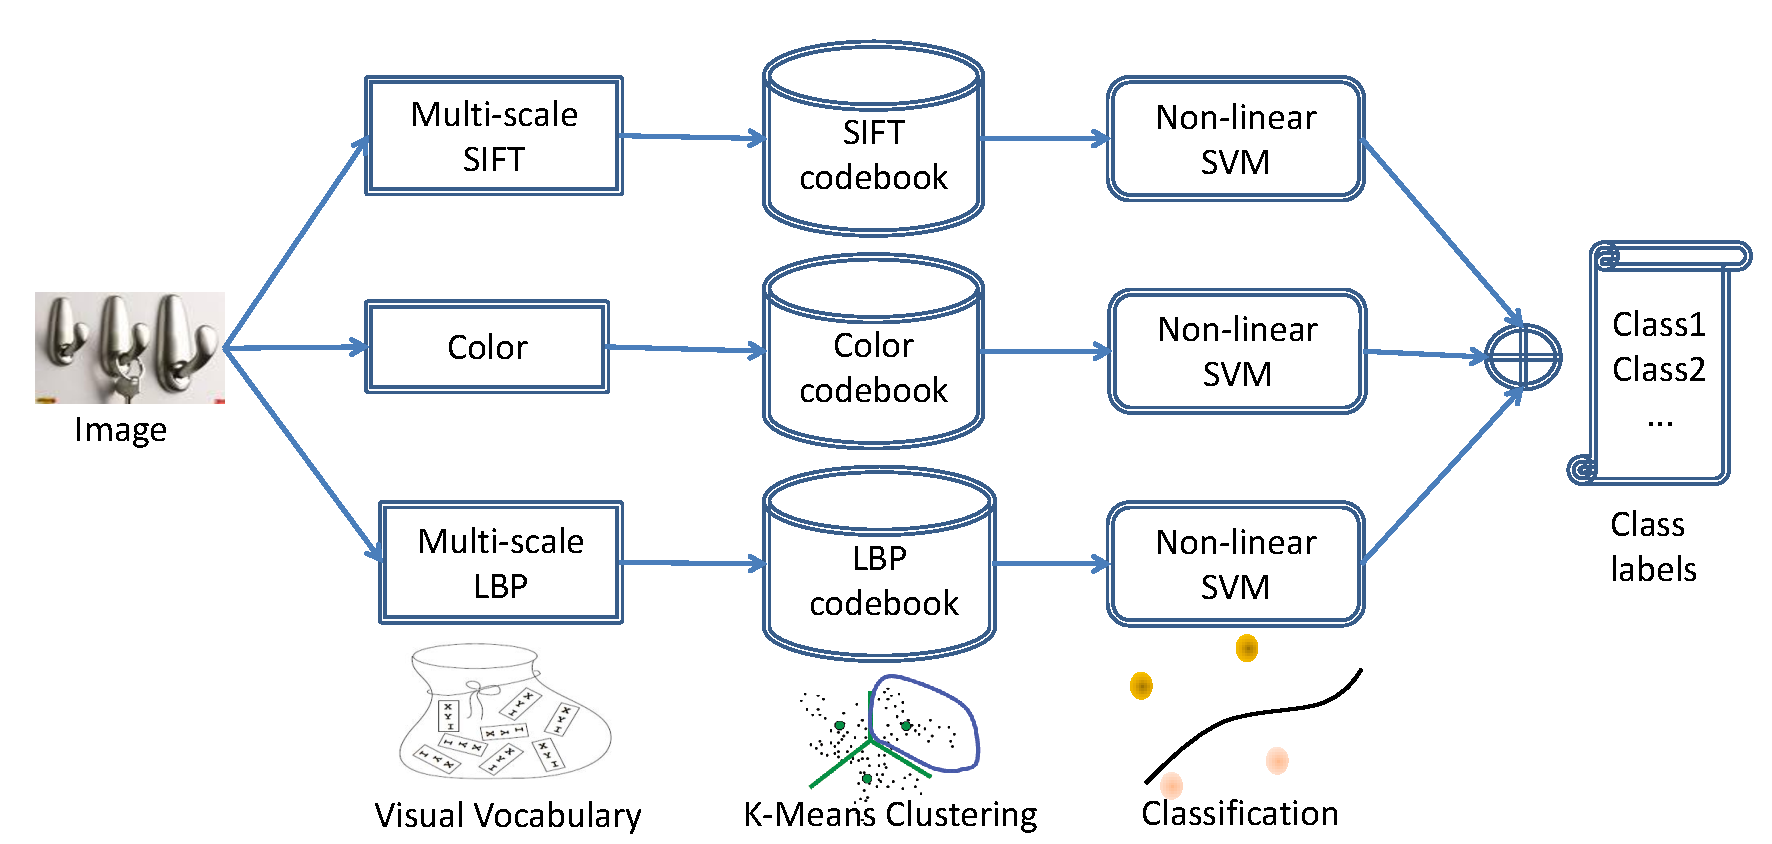
\includegraphics[width=1\textwidth]{flowchart}
\end{figure}
\end{frame}

% % % % % % % % % % % % % % % % 


\begin{frame}
\frametitle{Feature Descriptors}
\begin{columns}
\begin{column}{.3\textwidth}
\begin{block}{SIFT}
128 dimensions
\begin{figure}
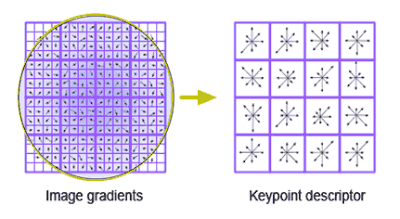
\includegraphics[width=\textwidth]{SIFT}
\end{figure}
16 orientation histograms, 8 bins each.
\end{block}
\end{column}
\pause
\begin{column}{.3\textwidth}
\begin{block}{LBP}
59 dimensions
\begin{figure}
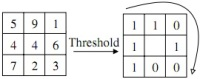
\includegraphics[width=\textwidth]{LBPSimple}
\end{figure}
\begin{figure}
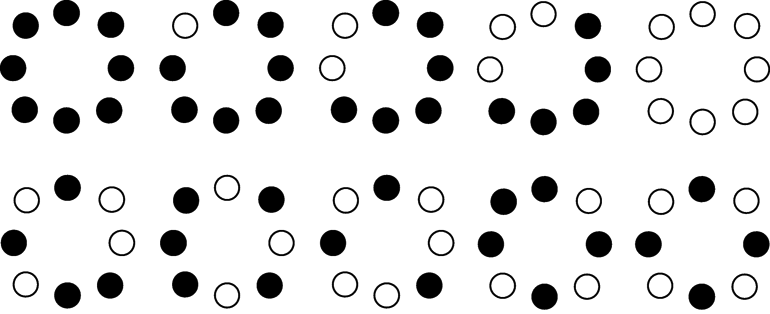
\includegraphics[width=\textwidth]{LBPU2}
\end{figure}
Compute histogram of the 59 ``U2'' patterns.
\end{block}
\end{column}
\pause
\begin{column}{.3\textwidth}
\begin{block}{RG}
64 dimensions
\begin{equation}
\begin{split}
R &= \frac{r}{r+g+b} \\
G &= \frac{g}{r+g+b} \\
\end{split}
\end{equation}
$R$ and $G$ each quantized into 32-bin histogram.
\end{block}
\end{column}
\end{columns}
\end{frame}

\begin{frame}
\frametitle{Multi-Scale Dense Feature Extraction}
\begin{columns}
\begin{column}{.5\textwidth}
\begin{figure}
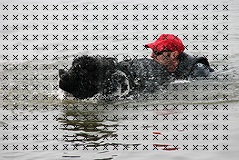
\includegraphics[height=1.5in]{dog_intdet}
\caption{Dense sampling at 3 scales}
\end{figure}
\end{column}
\pause
\begin{column}{.5\textwidth}
\begin{figure}
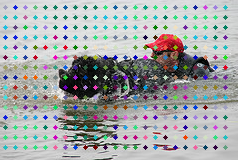
\includegraphics[height=1.5in]{dog_quantized}
\caption{Bag of words}
\end{figure}
\end{column}
\end{columns}
\end{frame}
%

% % % % % Classification slides % % % % % % % 
\begin{frame}
\frametitle{Classifiers}
\begin{itemize}
\item<1-3> Train three different SVM classifiers for each of the codebooks.\\
\item<2-3> Linear kernel does not work very well because the classes are not well separable in the feature space.\\
\item<3> Need to map the data to a higher dimensional space: \textbf{RBF kernel}.\\
\end{itemize}
\begin{figure}
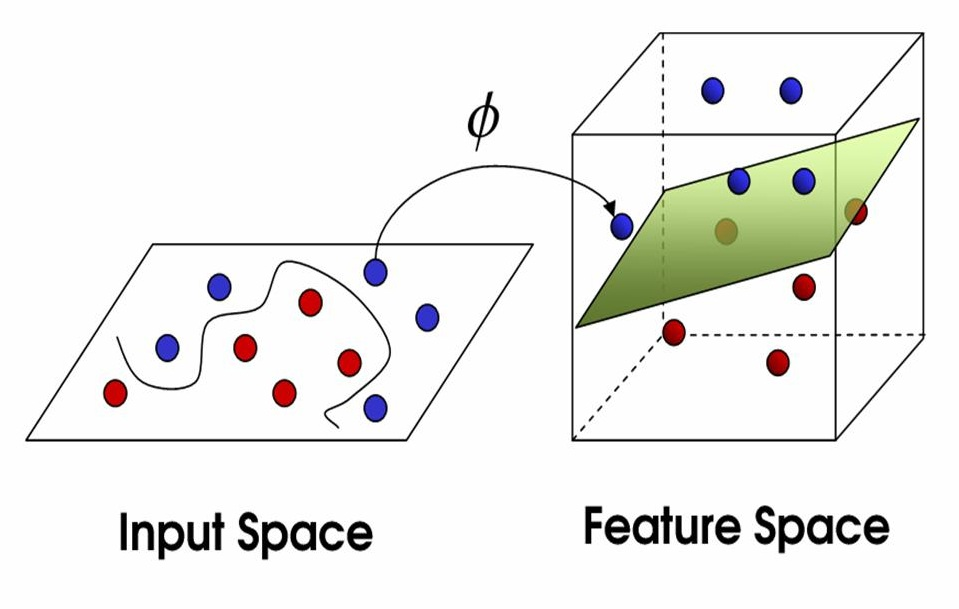
\includegraphics[width = 0.7\textwidth, height = 0.5\textheight]{svm}
\end{figure}
\end{frame}

\begin{frame}
\frametitle{Parameter Selection}
\begin{itemize}
\item<1-3> Effectiveness of SVM classifiers depends on the selection of the right set of parameters.
\item<2-3> Two different parameters for RBF-SVM: \textbf{soft margin parameter C} and \textbf{kernel width G}.
\item<3> Coarse-to-fine grid search (with 5 fold cross validation) for selecting the optimum set of parameters.
\end{itemize}
\begin{figure}
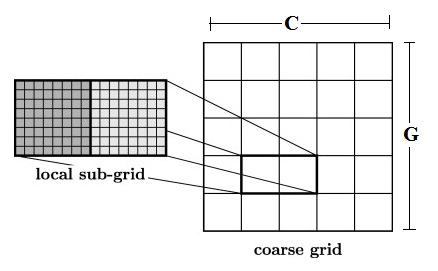
\includegraphics[width = 0.6\textwidth, height =0.4\textheight]{gridsearch}
\end{figure}
\end{frame}

\begin{frame}
\frametitle{Classifier Combination}
\begin{figure}
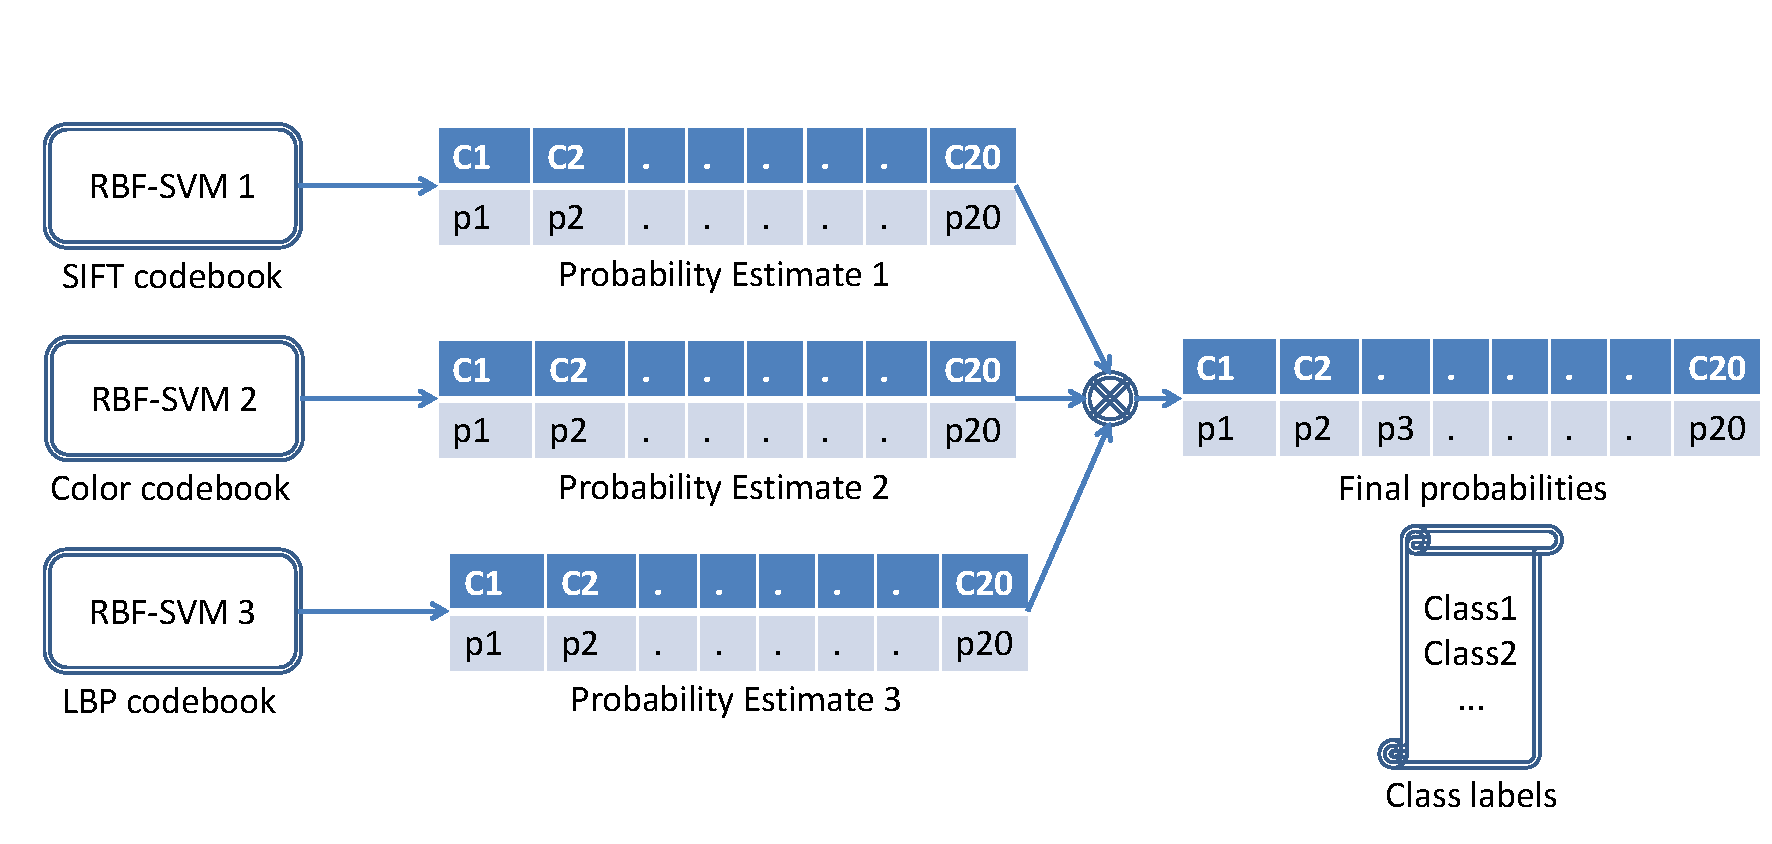
\includegraphics[width = 1\textwidth]{classifiercombination}
\end{figure}
\end{frame}

\begin{frame}
\frametitle{Results}
\begin{itemize}
\item<1-3> Classes where the approach really works well: \textit{odometer, rapeseed, website}.
\item<2-3> Classes where the approach does not work very well: \textit{lopener, hatchet, cleaver}.
\item<3> Top-5 accuracy:
\begin{itemize}
\item \textbf{Training Set}: 99.99\%
\item \textbf{Validation Set}: 88.55\%
\item \textbf{Test Set}: 88.94\%
\end{itemize}
\end{itemize}
\end{frame}

\begin{frame}
\frametitle{Success}

\only<1>{
\begin{figure}
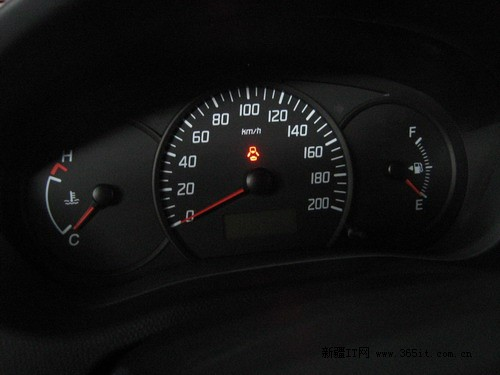
\includegraphics[width =0.4\textwidth, height =0.5\textheight]{success1}
\caption{\textbraceleft'odometer','spatula','gondola','hook','elocomotive'\textbraceright}
\end{figure}
}

\only<2>{
\begin{figure}
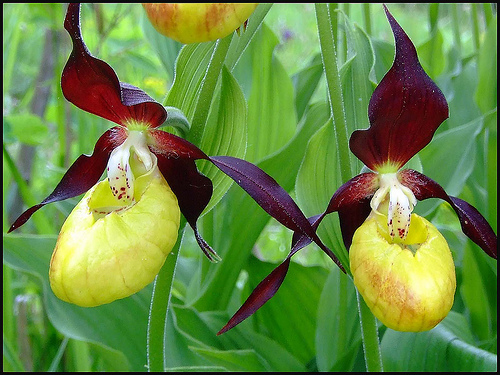
\includegraphics[width =0.4\textwidth, height =0.5\textheight]{success2}
\caption{\textbraceleft'yflower','daisy','flamingo','ladle','plunger'\textbraceright}
\end{figure}
}
\end{frame}


\begin{frame}
\frametitle{Failure}

\only<1>{
\begin{figure}
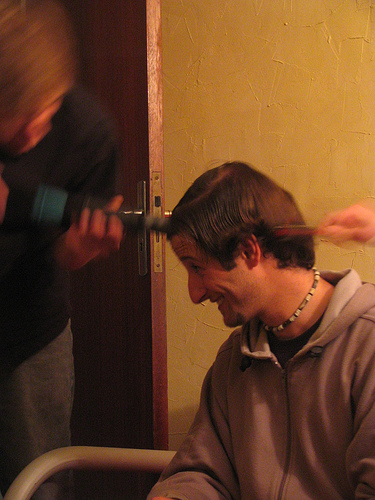
\includegraphics[width =0.4\textwidth, height =0.5\textheight]{failure1}
\caption{\textbraceleft'plunger','ladle','spatula','hook','cleaver'\textbraceright}
\end{figure}
}

\only<2>{
\begin{figure}
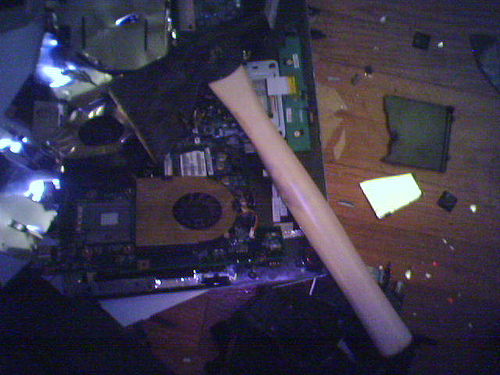
\includegraphics[width =0.4\textwidth, height =0.5\textheight]{failure2}
\caption{\textbraceleft'odometer','daisy','flamingo','ladle','spatula'\textbraceright}
\end{figure}
}
\end{frame}
% % % % % % % % % % % % % % % % % % % % % % %

%\begin{frame}[fragile] % Notice the [fragile] option %
%\frametitle{Verbatim}
%\begin{example}[Putting Verbatim]
%\begin{verbatim}
%\begin{frame}
%\frametitle{Outline}
%\begin{block}
%{Why Beamer?}
%Does anybody need an introduction to Beamer?
%I don't think so.
%\end{block}
%% Extra carriage return causes problem with verbatim %
%\end{frame}\end{verbatim} 
%\end{example}
%\end{frame}
% 
%\begin{frame}[fragile]  % notice the fragile option, since the body
%			% contains a verbatim command
%Example of the \verb|\cite| command to give a reference is below:
%Example of citation using \cite{key1} follows on.
%\end{frame}
% 
%\begin{frame}
%\frametitle{References}
%\footnotesize{
%\begin{thebibliography}{99}
% \bibitem[Label1, 2010]{key1} Author's name (1987)
% \newblock Title of the paper.
% \newblock \emph{Journal Name} 55(4), 765 -- 799.
%\end{thebibliography}
%}
%\end{frame}
 
\begin{frame}
\centerline{Questions?}
\end{frame}
% End of slides
\end{document} 